\section{Experimental Results}
\label{sec:result}

This section presents the experimental results and the answers to the RQs. More results are available at https://github.com/csresearcher27/s2lct$\_$project.

% \InputWithSpace{tables/test-results-table}
\InputWithSpace{tables/test-results-3-50-table}
% \InputWithSpace{tables/test-results-3-100-table}
% \InputWithSpace{tables/test-results-3-200-table}

\begin{figure}
    \centering
    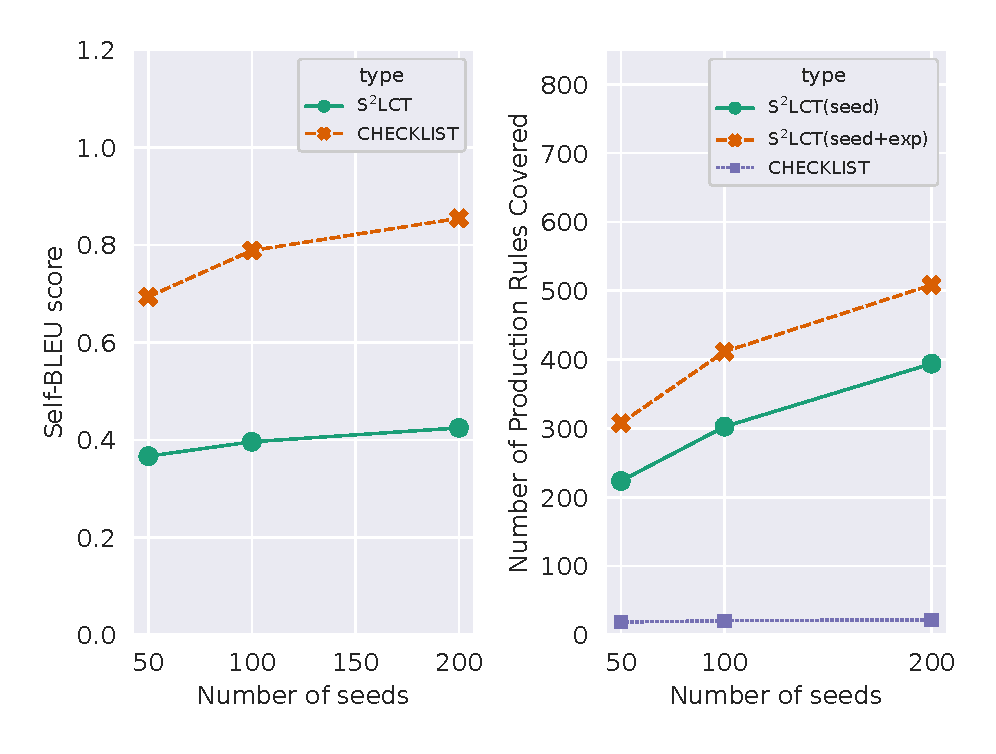
\includegraphics[width=0.35\textwidth]{figs/pdr-selfbleu-agg-lineplot.eps}
    \caption{\PdrSelfbleuFigCaption}
\end{figure}

% \begin{figure}%
%     \centering
%     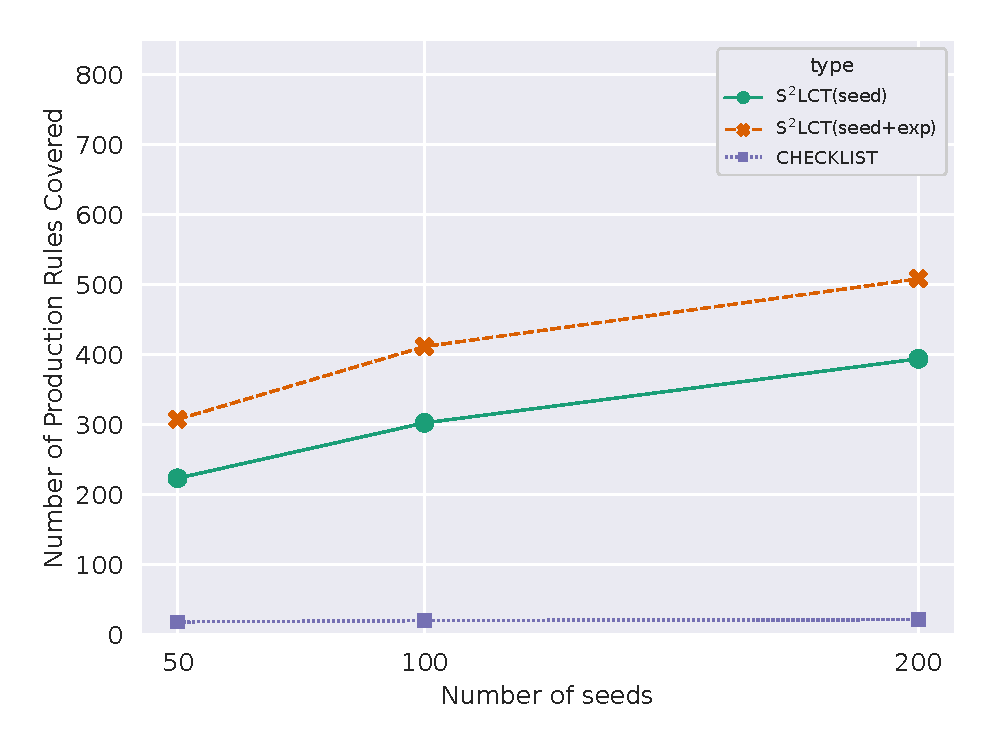
\includegraphics[width=0.35\textwidth]{figs/pdr-agg-lineplot.eps}
%     \caption{\PdrFigCaption}
% \end{figure}


% \begin{figure}%
%     \centering
%     \subfloat[][\centering\SelfbleuFigCaption]{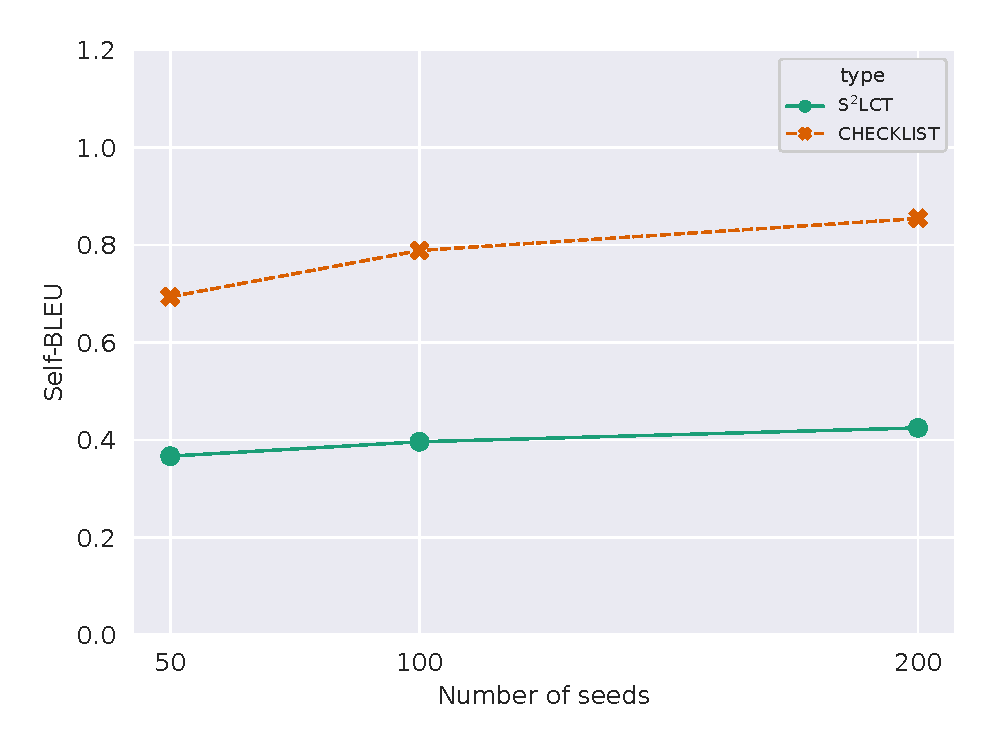
\includegraphics[width=0.35\textwidth]{figs/selfbleu-agg-sample-lineplot.eps}}%
%     \qquad
%     \subfloat[][\centering\PdrFigCaption]{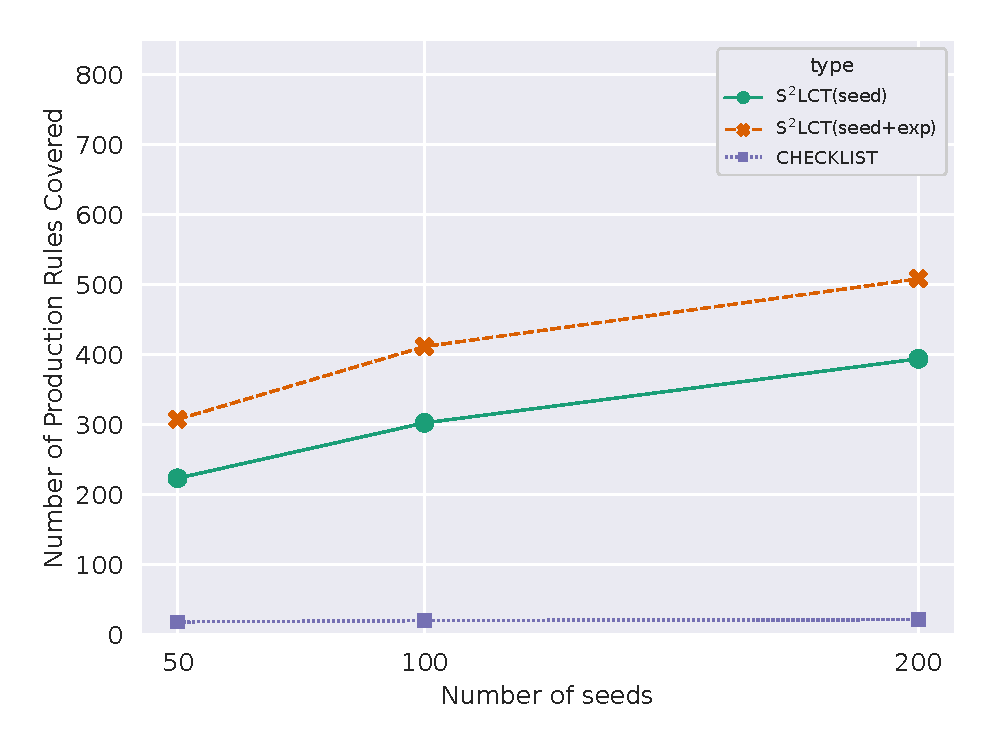
\includegraphics[width=0.35\textwidth]{figs/pdr-agg-lineplot.eps}}
%     \caption{\FailModelsFigCaption}
% \end{figure}

\begin{figure}%
    \centering
    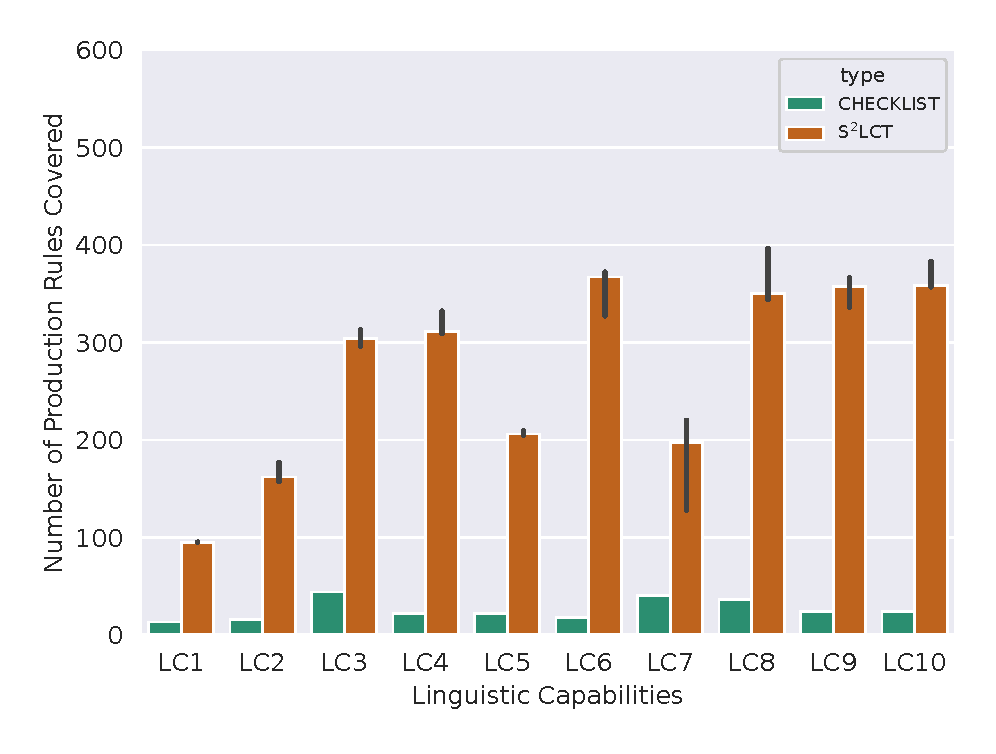
\includegraphics[width=0.35\textwidth]{figs/pdr-ours-50seeds-barplot.eps}
    \caption{\PdrBarplotFigCaption}
\end{figure}

\begin{figure}%
    \centering
    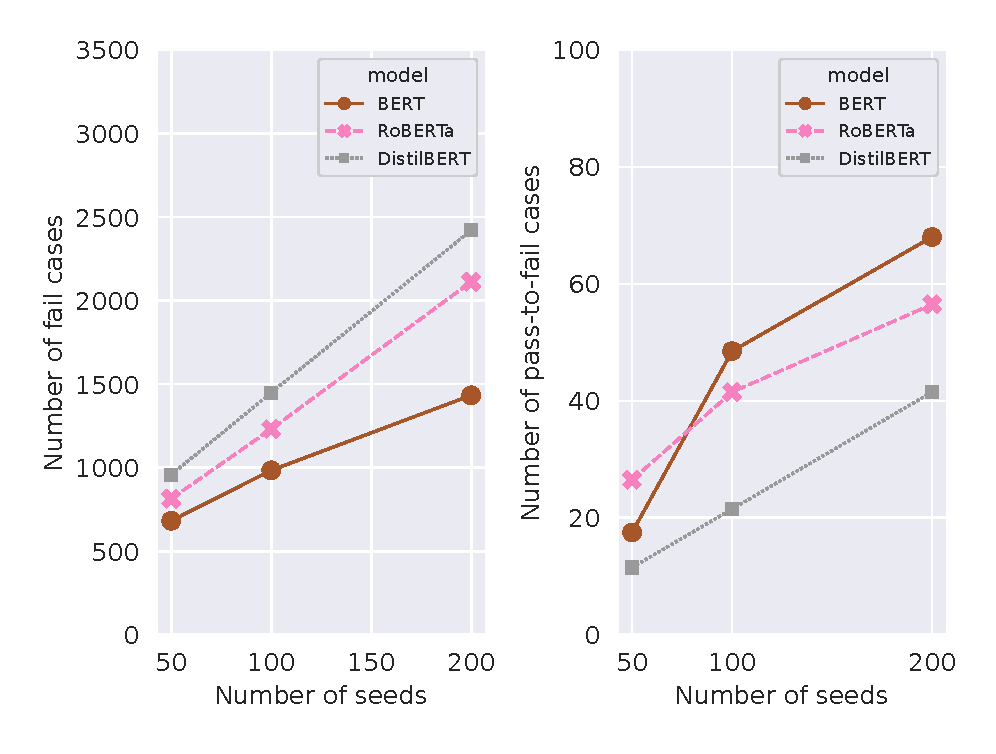
\includegraphics[width=0.35\textwidth]{figs/numfail-pass2fail-agg-lineplot.eps}
    \caption{\FailModelsFigCaption}
\end{figure}

% \begin{figure}%
%     \centering
%     \subfloat[][\centering\NumFailModelsSubFigCaption]{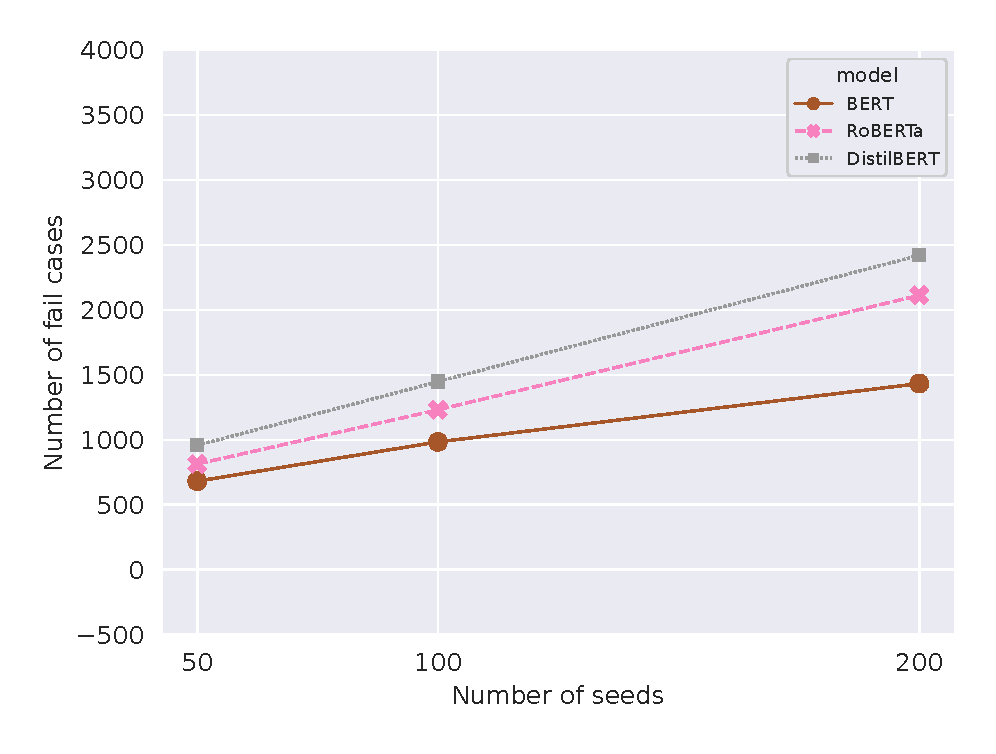
\includegraphics[width=0.35\textwidth]{figs/numfail-agg-lineplot.eps}}%
%     \qquad
%     \subfloat[][\centering\FailRateModelsSubFigCaption]{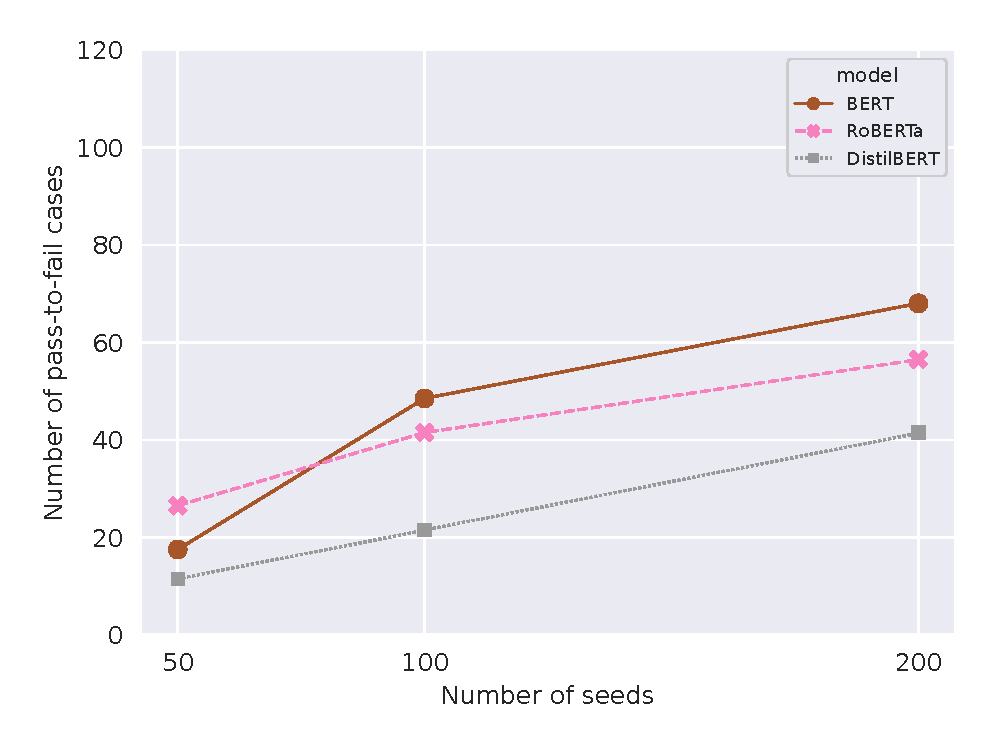
\includegraphics[width=0.35\textwidth]{figs/pass2fail-agg-lineplot.eps}}
%     \caption{\FailModelsFigCaption}
% \end{figure}

\subsection{RQ1: Test Case Diversity}

Our results show that \emph{\tool generated many test cases that the sentiment analysis models failed to predict the correct labels, and it produced significantly more diverse test cases than \Cklst did.}

\paragraph*{\selfbleu} Left in Figure~\ref{fig:PdrSelfbleu} compares the \selfbleu scores between \tool seed sentences and \Cklst test cases. The x-axis shows sizes of random samples of \tool seeds and \Cklst test cases, and y-axis shows the \selfbleu scores.
% Median value of \selcbleu scores are computed from randomly sampled seeds over 3 trials for each \lc,
Median of the \selfbleu scores over all \lcs is shown in left in figure \ref{fig:PdrSelfbleu}. We observe that \selfbleu scores of \Cklst test cases is significantly higher than those of \tool seeds, for all numbers of seeds. This result indicates \Cklst test cases are less diverse than \tool seeds, which demonstrates the benefit of searching from a real-world search dataset over creating test cases from limited number of preset templates.
% From the figure, we can observe that seed generation step in \tool generates more diverse text sentences than \Cklst.

\paragraph*{\Pdr} Right in figure~\ref{fig:PdrSelfbleu} compares \pdr between the \tool seed sentences, \tool seed and expanded sentences, and the \Cklst test cases. The x-axis shows the sizes of random samples of \tool seed sentences, \tool seed and expanded sentences, and \Cklst test cases, and y-axis shows the \pdr scores. Median of the \pdr scores over all \lcs is shown in the right in the figure~\ref{fig:PdrSelfbleu}. The figure \ref{fig:PdrSelfbleu} shows that \tool seed and/or expanded sentences produce significantly higher \pdr scores than \Cklst test cases did. Also, more \tool seeds cover more production rules.

Figure~\ref{fig:PdrBarplot} compares the \pdr between 50 \tool seeds and all \Cklst test cases for each \lc. The x-axis shows each one \lc, and the y-axis is the \pdr for these test cases.
% \tool test cases are generated from randomly selected 50 seeds, and the median value over 3 trials for each \lc is reported.
% It is observed that \tool covers significantly higher number of different syntactic production rules than \Cklst for all \lcs.
We observed that even with only 50 seeds in each \lc, \tool seeds cover significantly higher number of production rules than all \Cklst test cases (ranging from 95 for LC1 to 367 for LC6 for \tool seeds and from 13 for LC1 to 44 for LC3 for \Cklst seeds) in each \lc.
% (ranging from 4.92 times to 20.38 times higher scores for LC7 and LC6 respectively) 

Overall, the above results show that \tool test cases are significantly more diverse in terms of syntactic structure than \Cklst.

\paragraph*{Model Test Results} Table~\ref{table:TestResult} shows the testing results of the three NLP models on \tool test cases using 50 seeds. First column lists linguistic capabilities for the \sa task, and Column 2 shows the numbers of seed test cases, and Column 3 shows the median numbers of expanded test cases over 3 trials. Columns 4 and 5 show the median numbers of failed test cases and the failure rates (i.e., percentage of test cases that a model predicts incorrect labels) of each NLP models on the seed and expanded test cases over the 3 trials, respectively. Column 6 shows the median number of expanded test cases that failed, but their corresponding seed test cases passed over the 3 trials(\Ptf). We observe that in all \lcs, \tool produces hundreds of test cases, expanding at least an order of magnitude more test cases than the seeds. LC1 and LC5 have 19 and 26 seeds, respectively. This is because \tool's search rules and transformation templates of these two linguistic capabilities produced few seeds. Nevertheless, the syntax-base sentence expansion phase generated of 224 and 1090 test cases, respectively.
In terms of model performance, all three models achieve low failure rates in LC2 and LC9 while the failure rates are high in all other linguistic capabilities (13.52\%-99.95\%). We also observe that there are many expanded test cases that failed, but their corresponding seeds did not (last column). This shows that the syntax-based sentence expansion phase indeed introduces more diverse sentence structures in the test cases that cause the models to fail.

In addition, Figure~\ref{fig:FailModels} shows the numbers of fail and pass-to-fail cases with different number of seeds used. We observed that more \tool seeds introduce more failed cases and more \Ptf cases, demonstrating the benefit of using more seeds when resource permits.



\begin{figure}
    \centering
    \includegraphics[width=0.5\textwidth]{figs/covergae.pdf}
    \caption{The coverage results of the generated test
      samples. \sw{Make the figures larger.}}
    \label{fig:coverage}
\end{figure}


Fig. \ref{fig:coverage} shows the coverage results of the generated
test samples, where the red line represents \tool and the black line
represents \Cklst.  Each column in Fig. \ref{fig:coverage} represent
the results for one NLP model, the first row is the \textit{BoundCov}
results and the second row is the \textit{SActCov} results.  From the
results, we make two observations observations. First, for \emph{all}
experimental settings (\eg NLP model, coverage metric), \tool achieves
high coverage than \Cklst. Recall that a higher coverage implies the
test case in the test suite is more diverse and rarely to have a
statistical distribution similar to the model training data. As a
result, a test suite with greater coverage complements the model
training data distribution (\ie hold-out testing data) better.  The
experimental results confirm that \tool can generate more diverse test
cases to complement the hold-out testing data for testing NLP models.
\sw{What does the growth trend in each figure indicate?} \sw{Does the
  absolute numbers or relative difference of the two lines on y axis
  mean anything concrete? E.g., how significant is the improvement in
  diversity?}

Another interesting finding is that for each NLP model, there is no
fixed relationship between \textit{BoundCov} and \textit{SActCov}. In
other words, while a test suite may produce higher \textit{BoundCov}
for some models, the same test suite may get higher \textit{SActCov}
for other NLP models.  Recall that \textit{BoundCov} measures both the
upper and lower corner neurons and \textit{SActCov} measures only the
upper corner neurons.  Such observation implies that the upper and
lower corner neurons are distributed unevenly, and measuring only one
of them is not enough.


\InputWithSpace{tables/manual-study-table}

\subsection{RQ2: Correctness of Sentiment Labels}
Table~\ref{table:ManualStudy} shows results of our manual study. The first column distinguishes the seed and expanded sentences. The number of test cases used for the study is represented in the
second column. The label consistency score defined
in Equation~\ref{metric:srel} is shown in column 3.

We observe that \emph{\tool generates test cases that consistently
  label their sentiment correctly.}  Column 3 shows that the label
consistency scores are 0.83 and 0.84 for the seed and expanded
sentences, respectively.
This means that \tool generates test oracles consistent with
human understanding most of the time. Also, there is
little difference of the scores between the seed and expanded
sentences. This implies that the syntax-based sentence expansion in
\tool preserves the sentiment as its seed.

% \sw{This paragraph is problematic. We are saying the inconsistency is just caused by human, indicating our tool is always correct?} Nevertheless, there exist inconsistency between \tool and manual labels. The causes of inconsistency are twofold. First, complicated sentences have led the participants to
% misunderstand its meaning. Second, phrase in a sentence has
% multiple interpretations of its sentiment. For example, the
% word ``easy'' could be interpreted as both compliment and back-handed
% insult.  
%% \sw{What are
%%   the causes of inconsistency? Looks like the main source of
%%   inconsistency comes from seed generation? Any insights on how it
%%   happened (e.g., issue with original labels, search rules, or
%%   templates?}

\subsection{RQ3: Correctness of Linguistic Capability Categorization}

The \lc relevancy score defined
in Equation~\ref{metric:lcrel} is shown in Column 4 of Table \ref{table:ManualStudy}. The result shows that
\emph{\tool generates test cases that are correctly categorized to the corresponding linguistic capabilities most of the time.}
The \lc relevancy scores for the seed and expanded sentences are both 0.9, achieving high order of agreement with human assessment. The fact that the expanded sentences
generated by \tool also have the same level of \lc
relevancy as the seed sentences shows that the syntax-based sentence expansion retains the linguistic capabilities.


\section{Application of \tool}
% \item \label{rq:four}: \textbf{Usefulness of Test Inputs.} 

In this section, we use one case study to show  \tool can be useful to help developers to find root causes of bugs in the \sa models.

\begin{figure*}
    \centering
    \includegraphics[width=0.8\textwidth]{figs/explain.pdf}
    \vspace{-4mm}
    \caption{Visualization of the buggy reason of two \tool generated test cases.}
    \label{fig:explain}
\end{figure*}


\MyPara{Experimental Process}
we conduct experiments to demonstrate that \tool can help developers understand the bugs in the NLP models.
Recall that \tool generates test cases by mutating seed sentences (\eg by expanding one token in the seed input). Still, it is unclear why mutating one token will cause the model to produce misclassified results.
We seek to help developers understand why such mutation will result in the misclassification. 
Existing work \cite{simin2020denas, lemna, lime} has demonstrated that the ML model prediction is dominated by a minimal set of input features (\ie tokens in input sentences). Motivated by such intuition, we identify a minimal set of input tokens that dominate the model prediction.

Formally, given a input sentence $x = [tk_1, tk_2, \cdots, tk_n]$, and the NLP model under test $f(\cdot)$, our goal is to find a masking template $T = [t_1, t_2, \cdots, t_n]$, where $t_i$ is 0 or 1, representing masking the $i^{th}$ token (\ie $tk_i$) in $x$ or not.
The template $T$ can mask some tokens in $x$ with attribute tokens, and the masked input has a high probability of retaining the original prediction $x$, denoted as
\begin{equation}
    P(f(T(x)) = f(x)) \ge P_{thresh}
    \label{eq:prob}
\end{equation}
To create such a template $T$, we first compute the contribution score of each input token using an existing explainable ML technique \cite{lemna}. We then begin with the full mask template (\ie, all tokens are masked); such full mask template definitely does not satisfy Equation \ref{eq:prob}.
We then iteratively shift one position from mask to non-mask based on the order of each token's contribution score, until the template $T$ satisfies Equation \ref{eq:prob}.
Because we iterate the size of the mask, the generated template $T$ will keep the minimum number of tokens in $x$. Moreover, since the input $x$ is an incorrect prediction, the generated template $T$ is likely to produce misclassification (i.e., the probability to be misclassified is larger than $P_{thresh}$).

\MyPara{Results} We generate a template that dominates the NLP model prediction to assist developers in understanding the false predictions. Figure \ref{fig:explain} shows the generated templates for two randomly selected seeds and their corresponding expanded test inputs.
The first example tests ``sentiments in (question, yes) form'' (LC9), and the second example tests ``negative positive with neutral content in the middle''  (LC7).
The first column shows the seed sentence, the second shows the expanded sentence, and the third shows each token's contribution score. The blue bar indicates the score for seed inputs, whereas the orange bar reflects the score for the expanded sentences.
We highlight the mutated token with yellow background and generated templates with red text. 

The results show that after mutating the seed sentence with one token, the token set that dominates the NLP model prediction has changed.
We can trace the root causes to the bias of the training data on the \lc under test; as a result, for the \lc under test, the model has a bias towards positive/negative for certain token sequence patterns. For example, LC9 has a bias toward the token sequence pattern that includes "maybe .... but ... even... yes". Thus, adding the token ``even" to the seed sentence will match one of those biased sequence patterns.
Sentences with such pattern in the training dataset are dominantly positive; thus, the models make the wrong decision on the sentence with ``even'' as positive. 
The visualization of each token's contribution score in the third column confirms our observation. Once ``even'' is added, scores of other tokens such as ``but'' and ``yes'' all change from negative to positive.
To fix the issue for LC9, we need to add more negative training samples with the format of ``maybe . .. but ... even ... yes''.
%he experimental results in Fig. \ref{fig:explain} illustrate that \tool can help developers to understand the buggy reason of the misclassification go no在,